\begin{figure}[H]
    \centering
    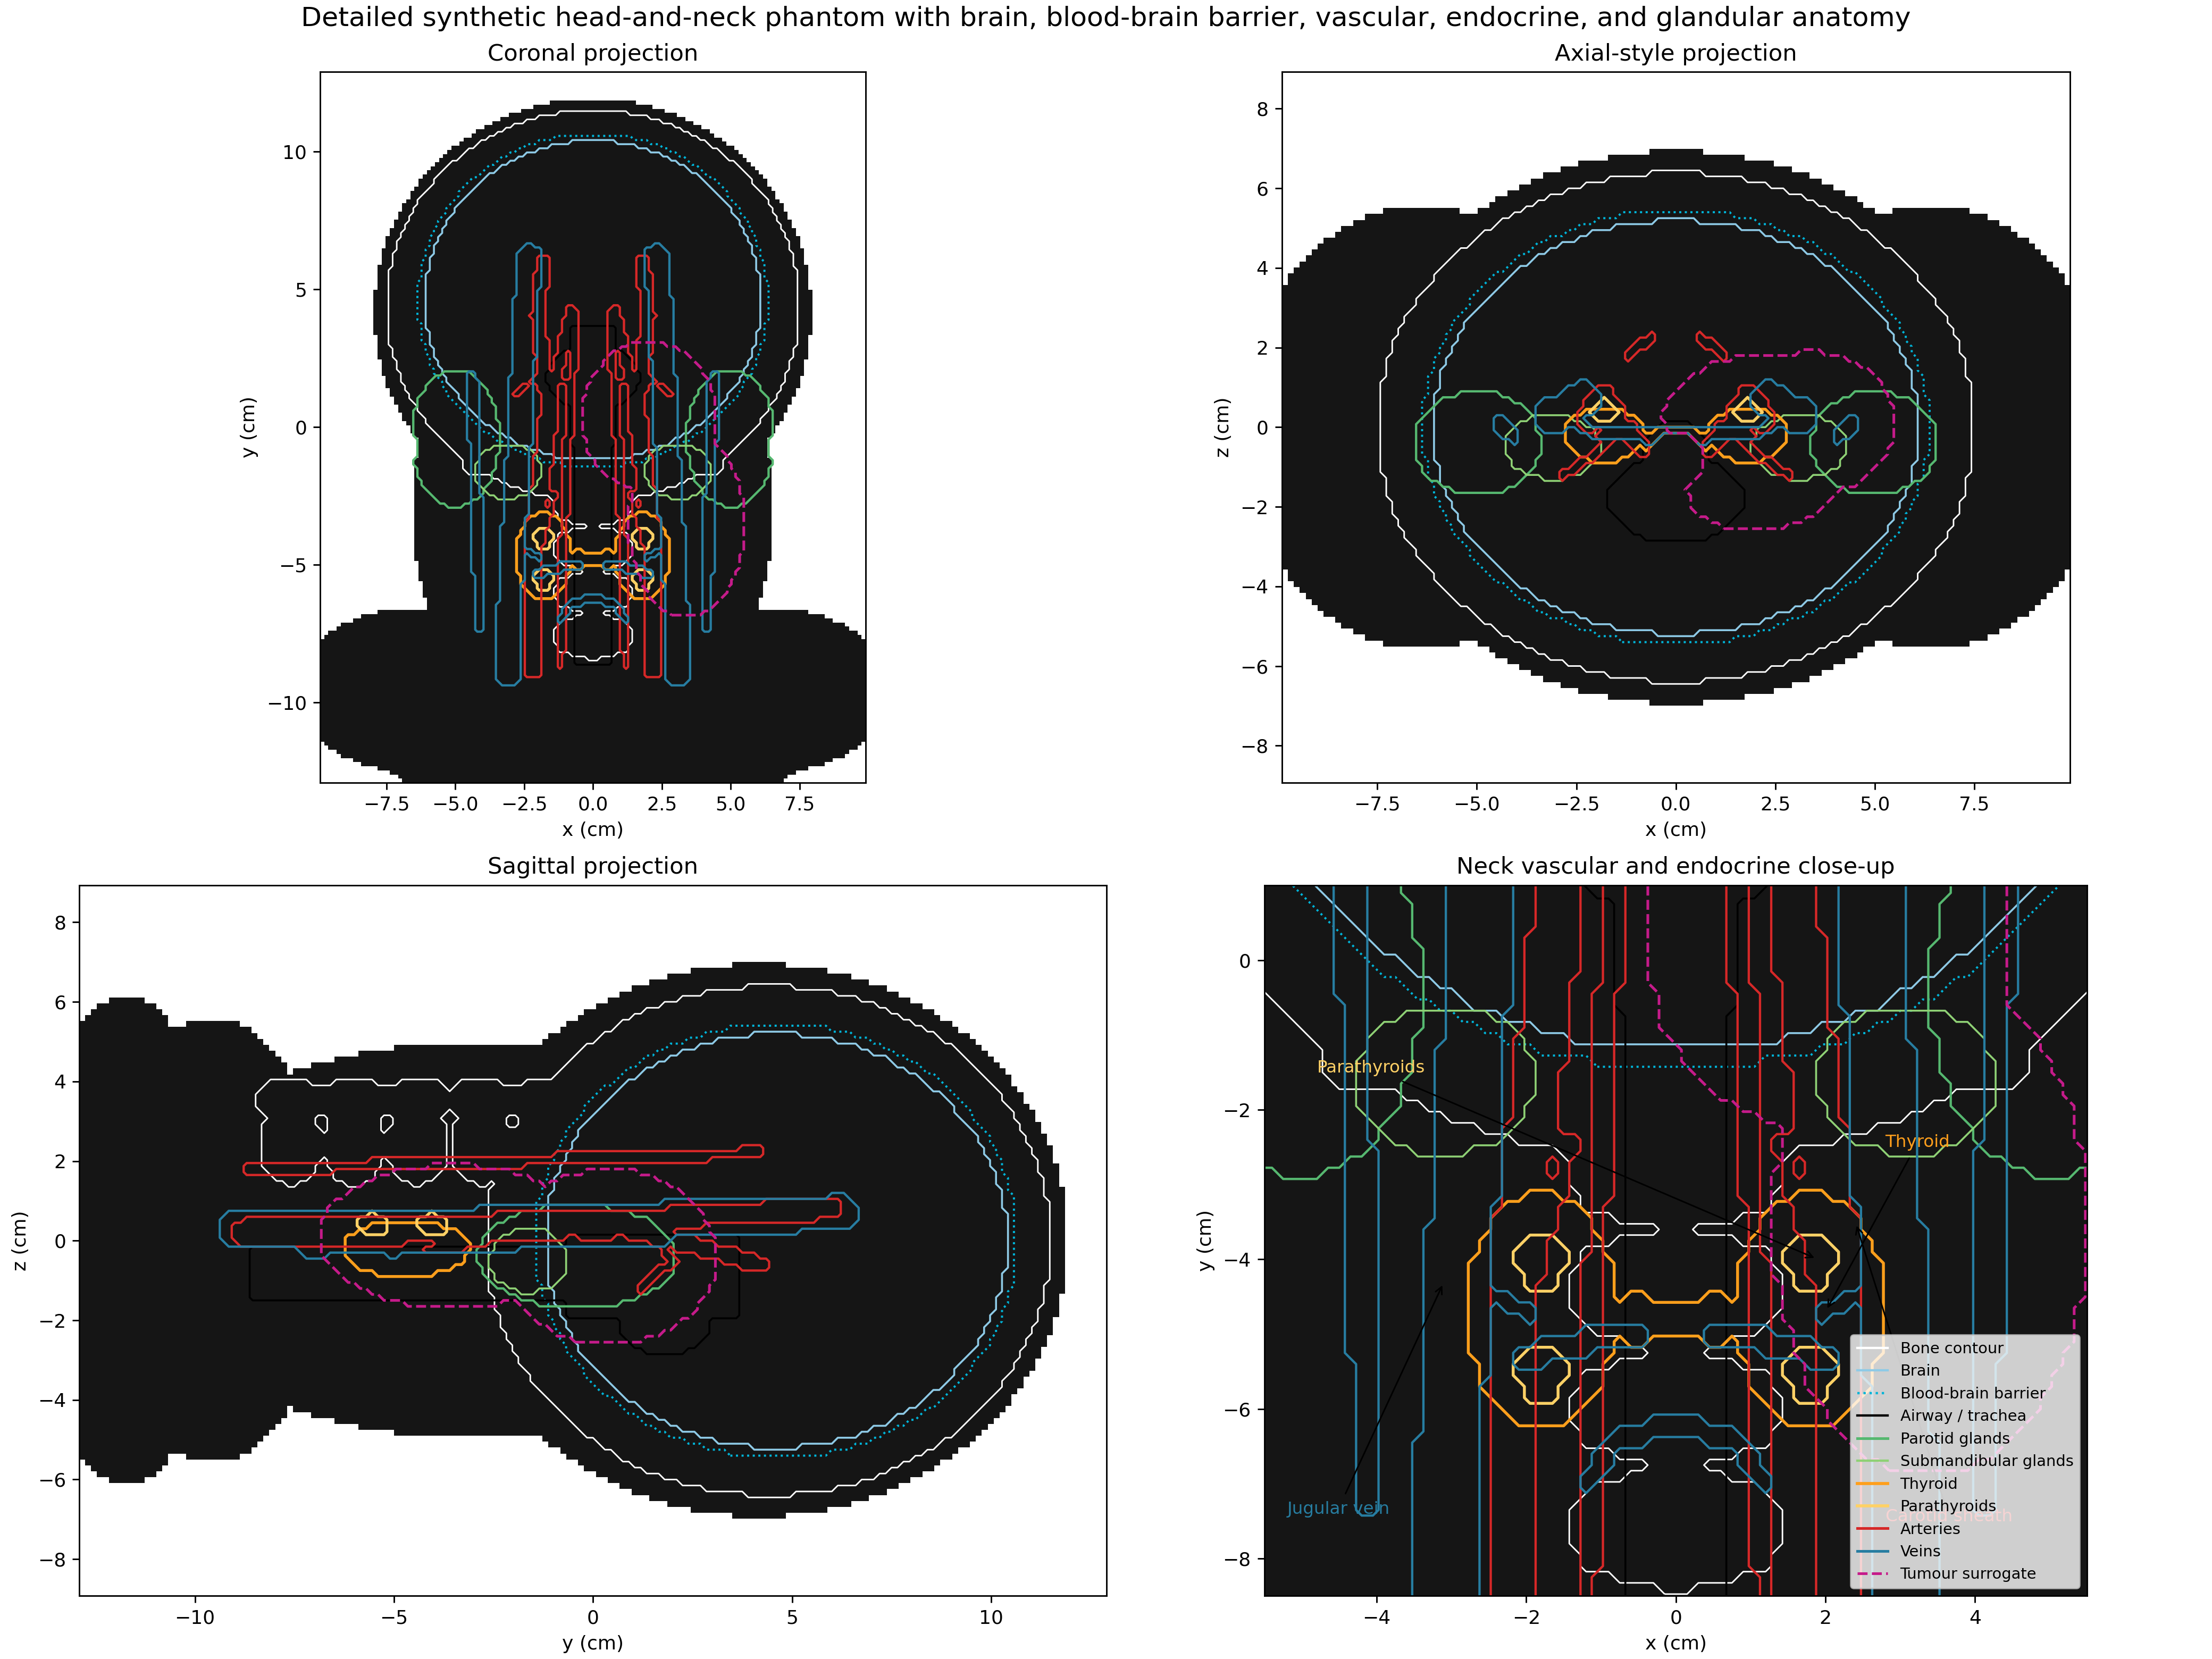
\includegraphics[width=\linewidth]{figureM1_voxel_phantom_anatomy.png}
    \caption{\textbf{Detailed synthetic voxelized head-and-neck phantom used for SFRT planning.} Multi-planar projections show the external contour and embedded anatomical structures, including the brain, BBB shell, thyroid-parathyroid complex, salivary glands, cervical spine, major arterial and venous pathways, and the bulky right-sided primary-plus-nodal tumour surrogate.}
    \label{fig:voxel_phantom_anatomy}
\end{figure}

\begin{figure}[H]
    \centering
    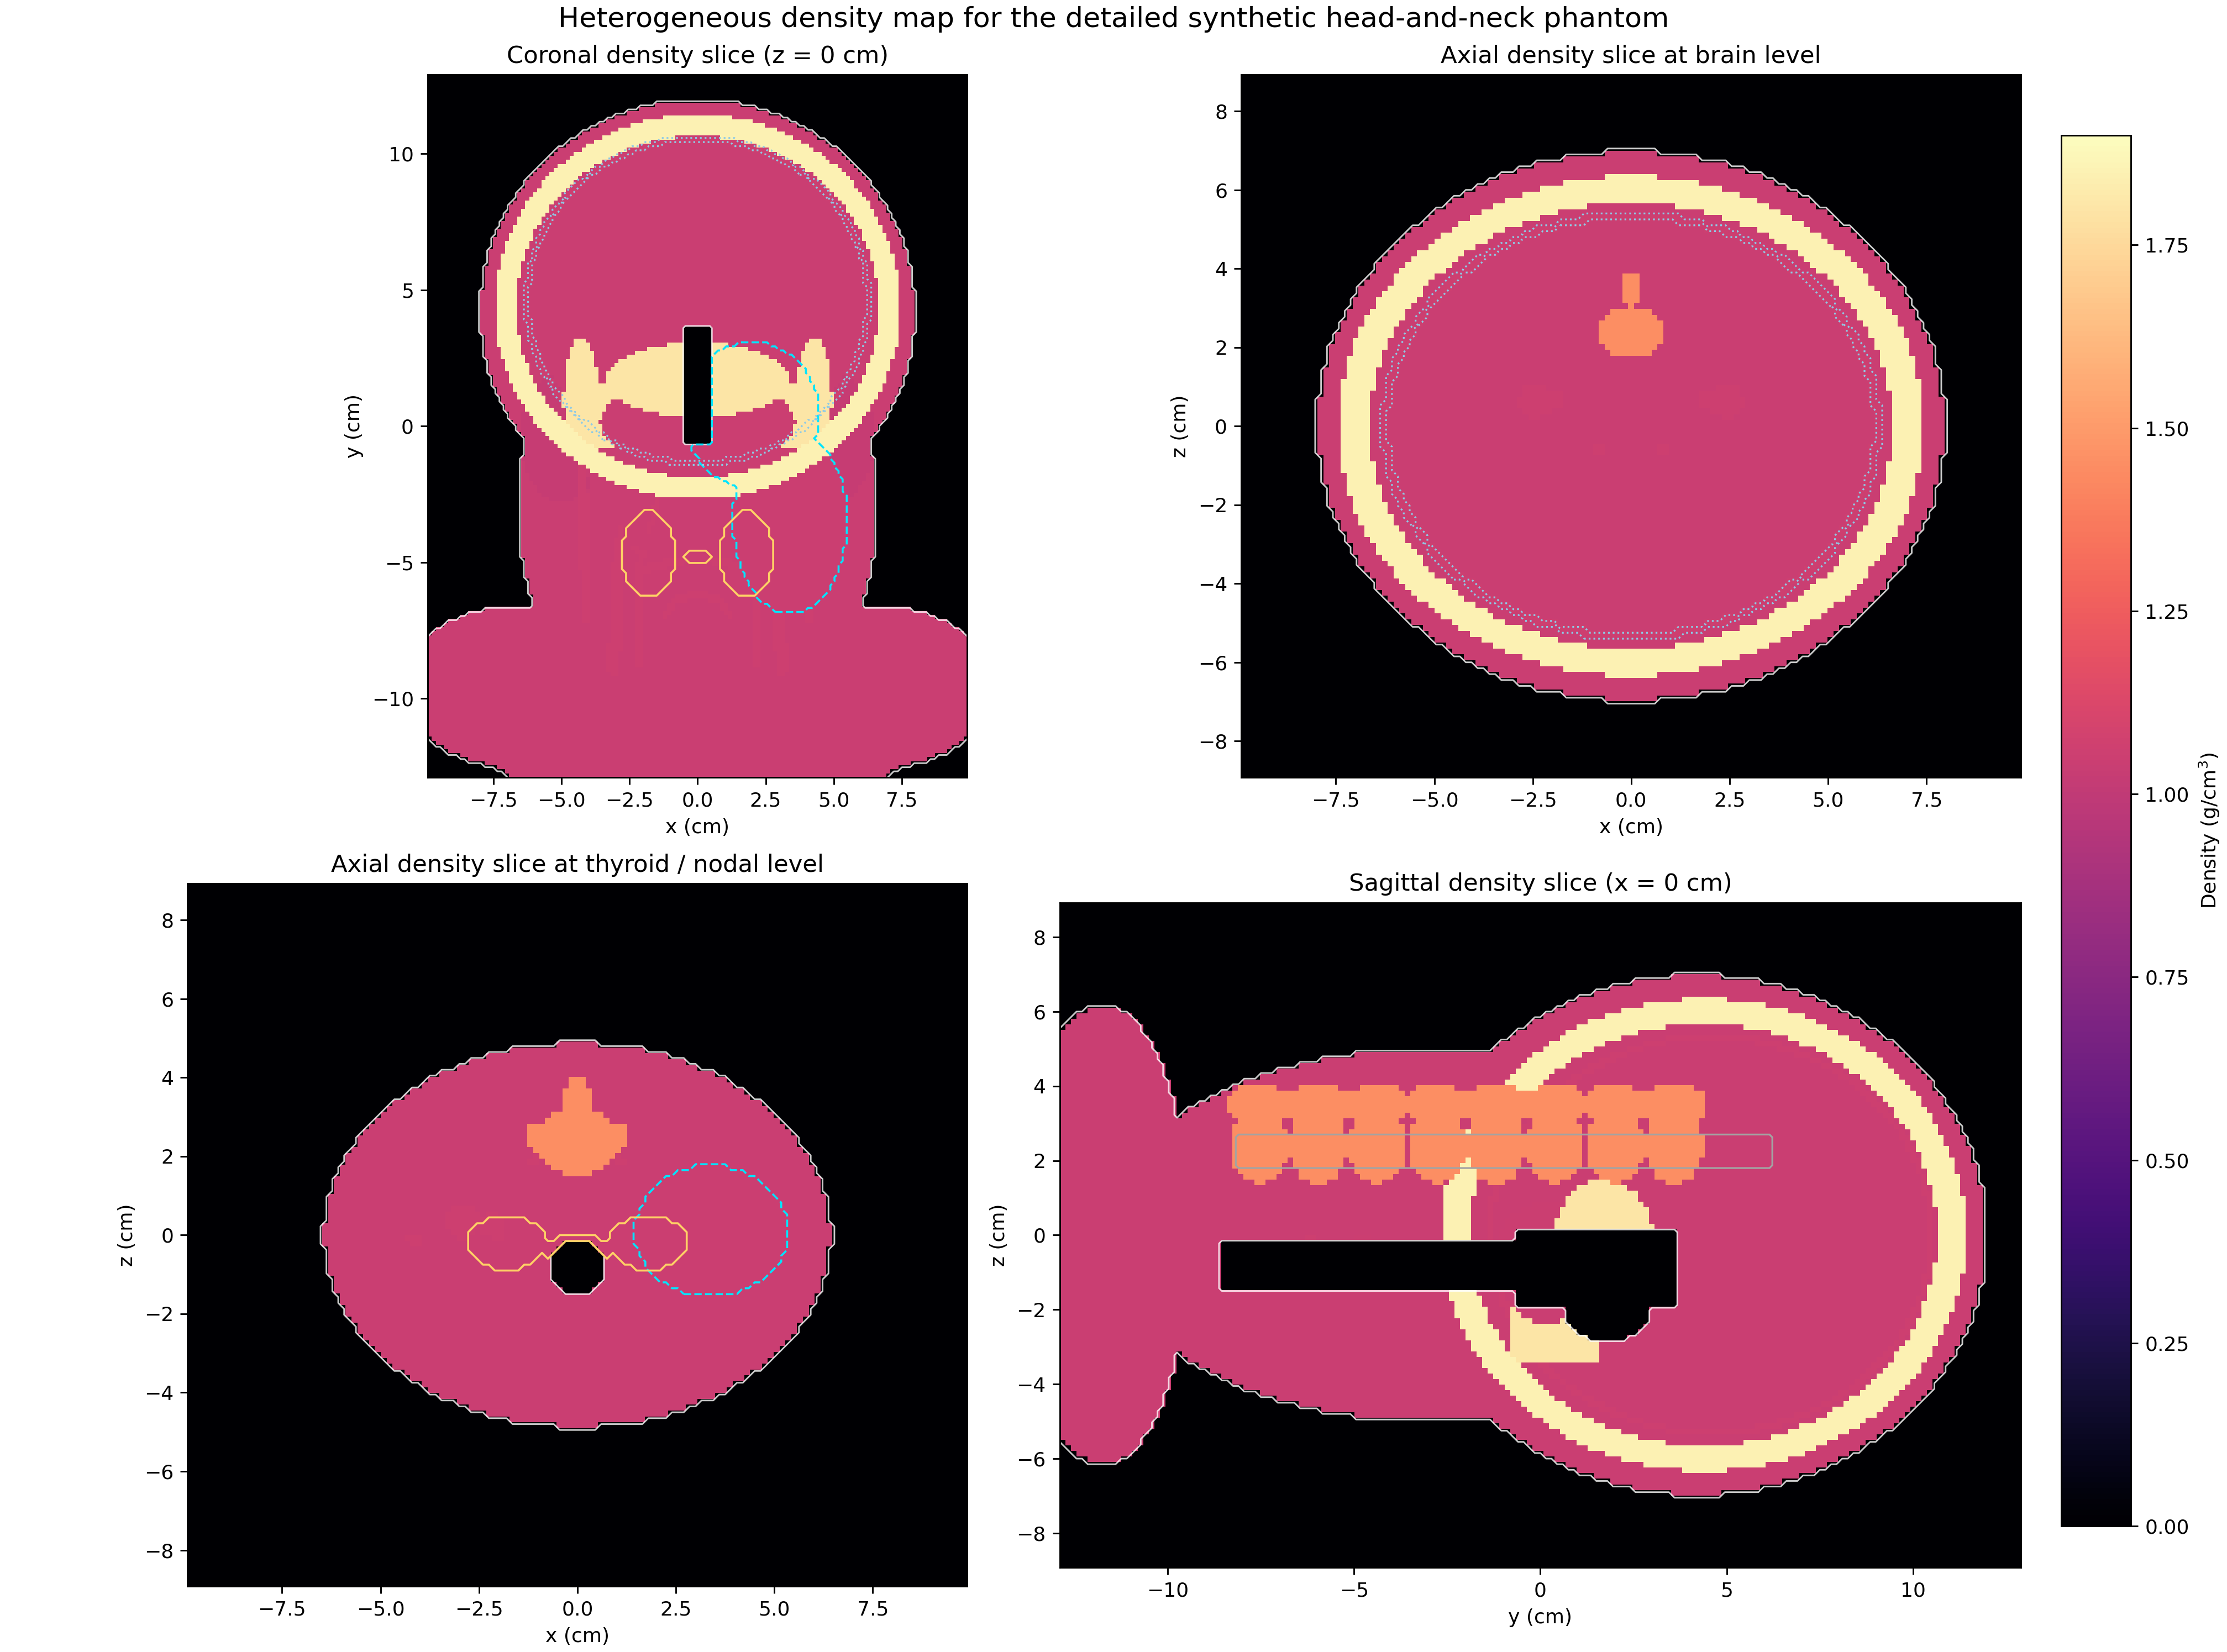
\includegraphics[width=\linewidth]{figureM2_voxel_phantom_density_map.png}
    \caption{\textbf{Bulk-density map of the voxelized head-and-neck phantom.} Representative coronal, axial, and sagittal views show the assigned density heterogeneity used to construct the TOPAS ImageCube dose-calculation phantom.}
    \label{fig:voxel_phantom_density}
\end{figure}

\begin{figure}[H]
    \centering
    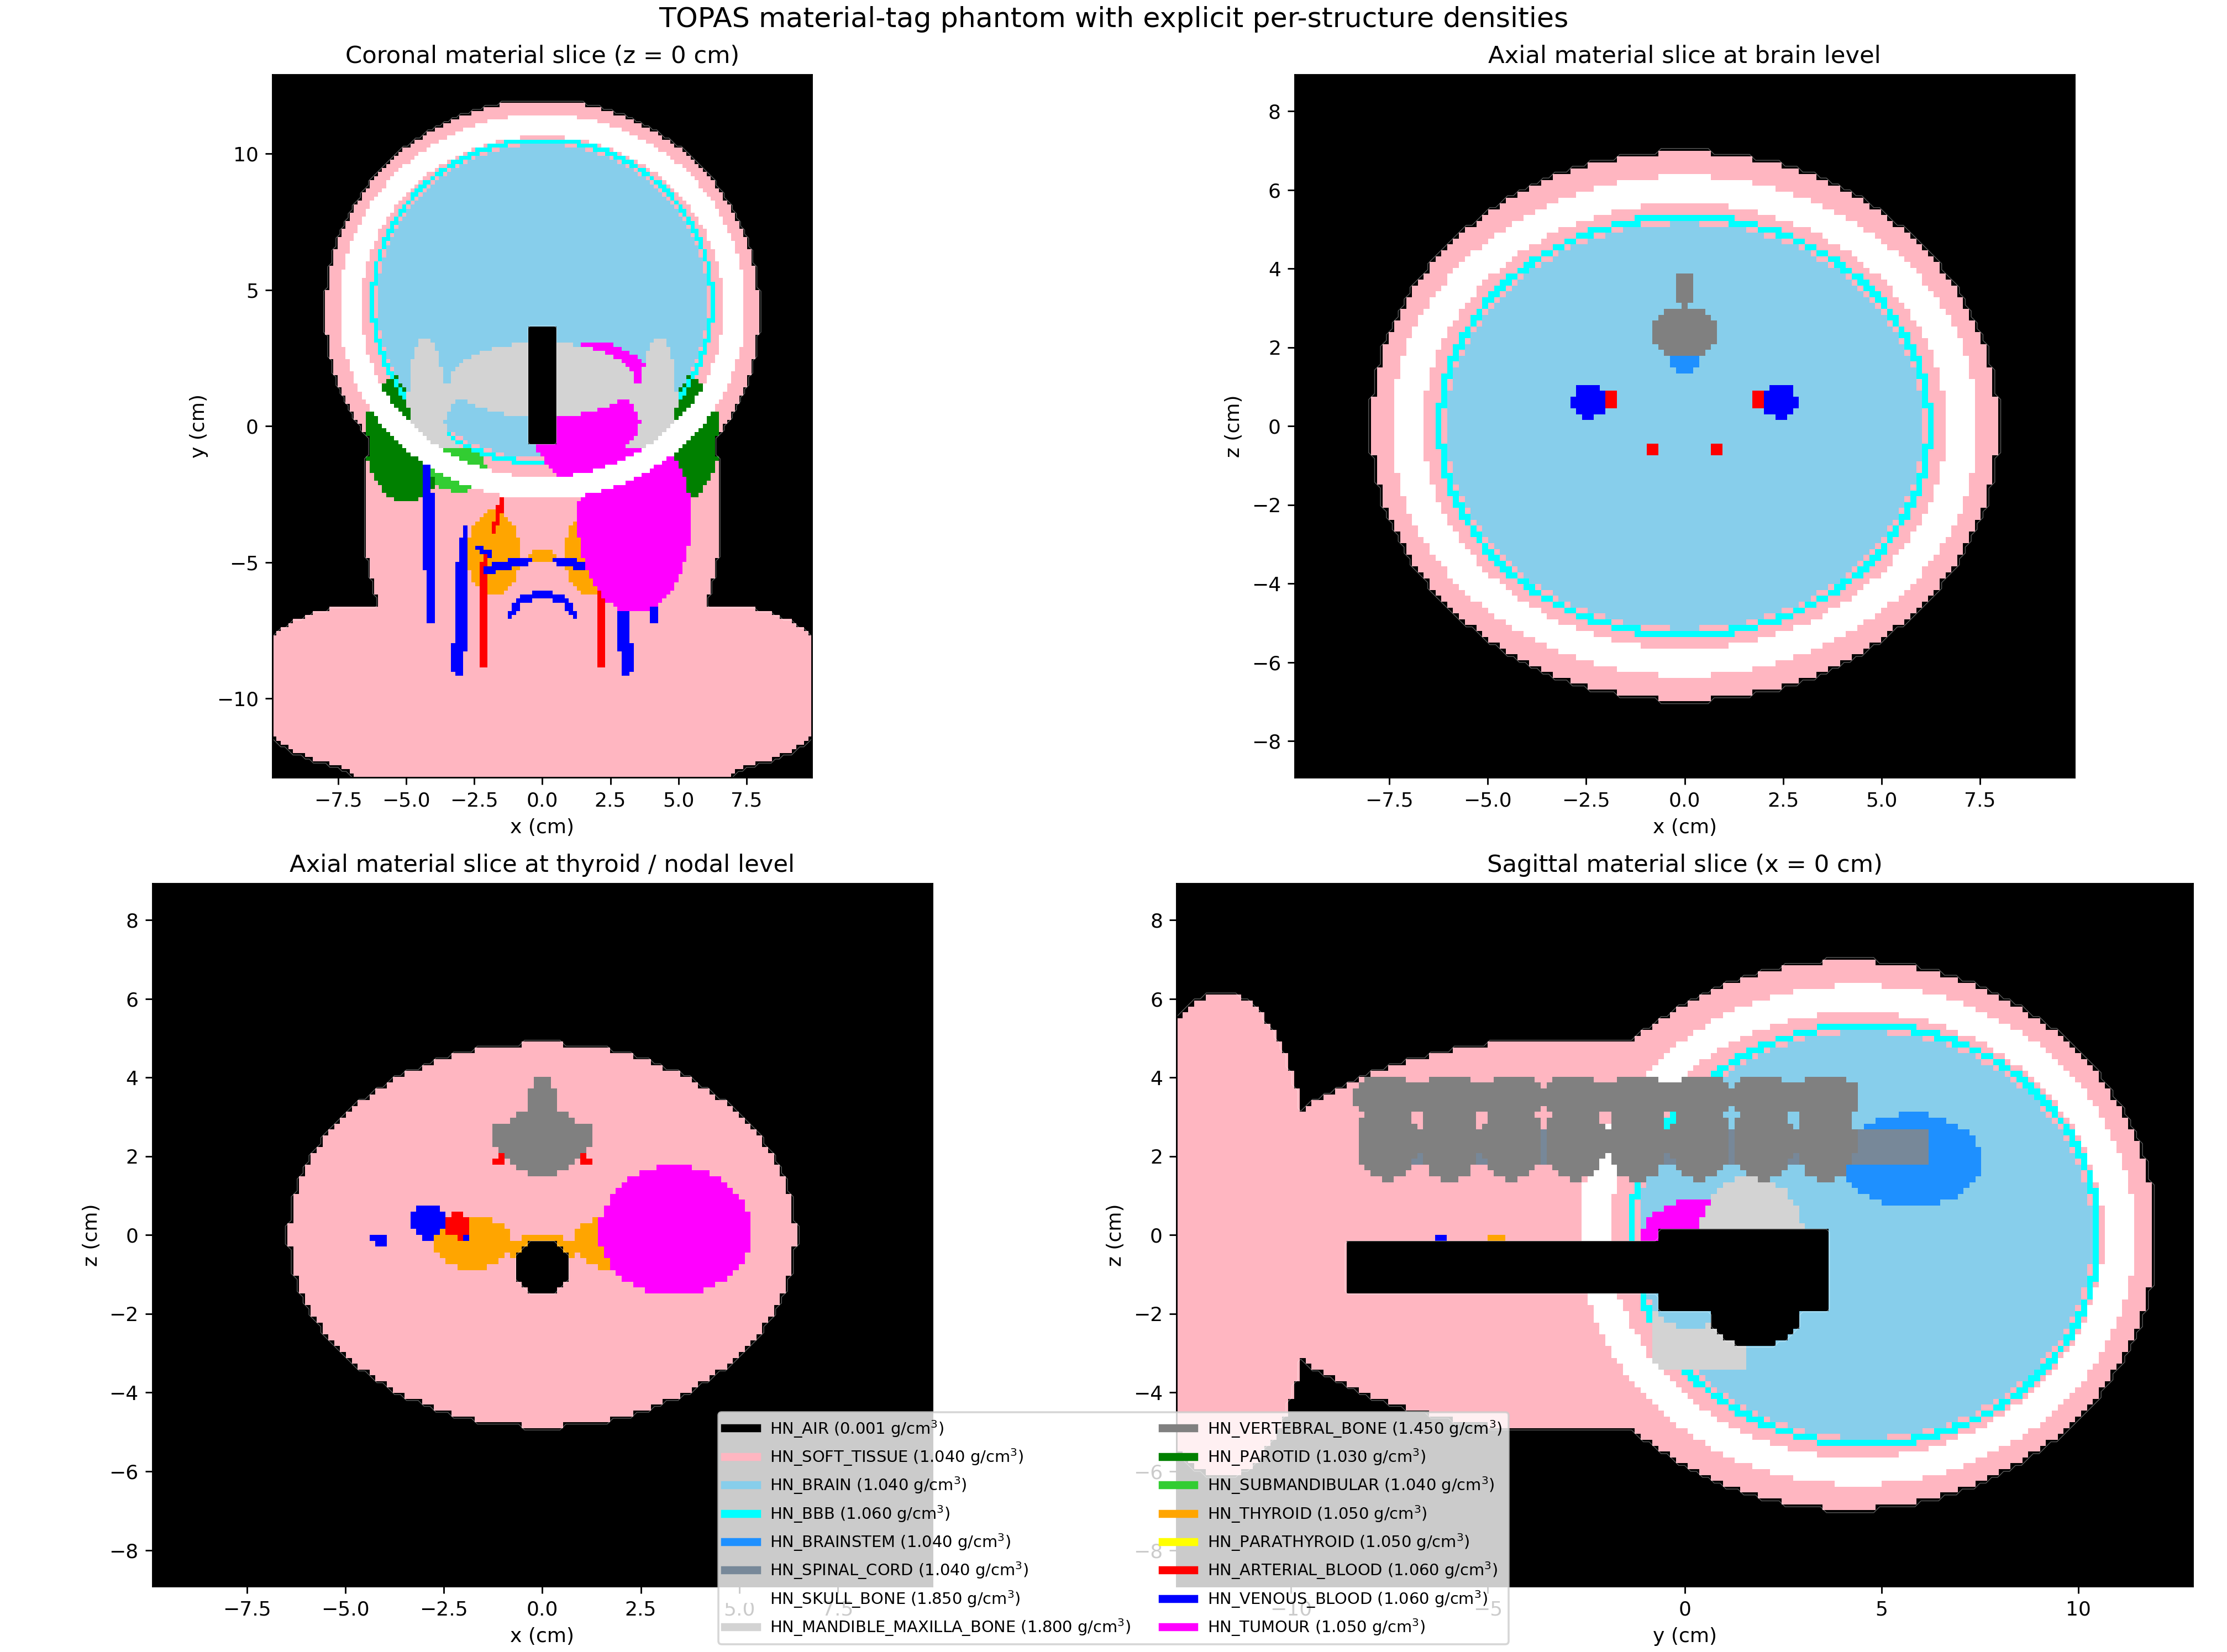
\includegraphics[width=\linewidth]{figureM3_topas_material_phantom.png}
    \caption{\textbf{TOPAS materialized voxel phantom.} Each anatomical compartment was converted into a discrete material tag linked to a Geant4 base material and explicit bulk density.}
    \label{fig:topas_material_phantom}
\end{figure}

\begin{figure}[H]
    \centering
    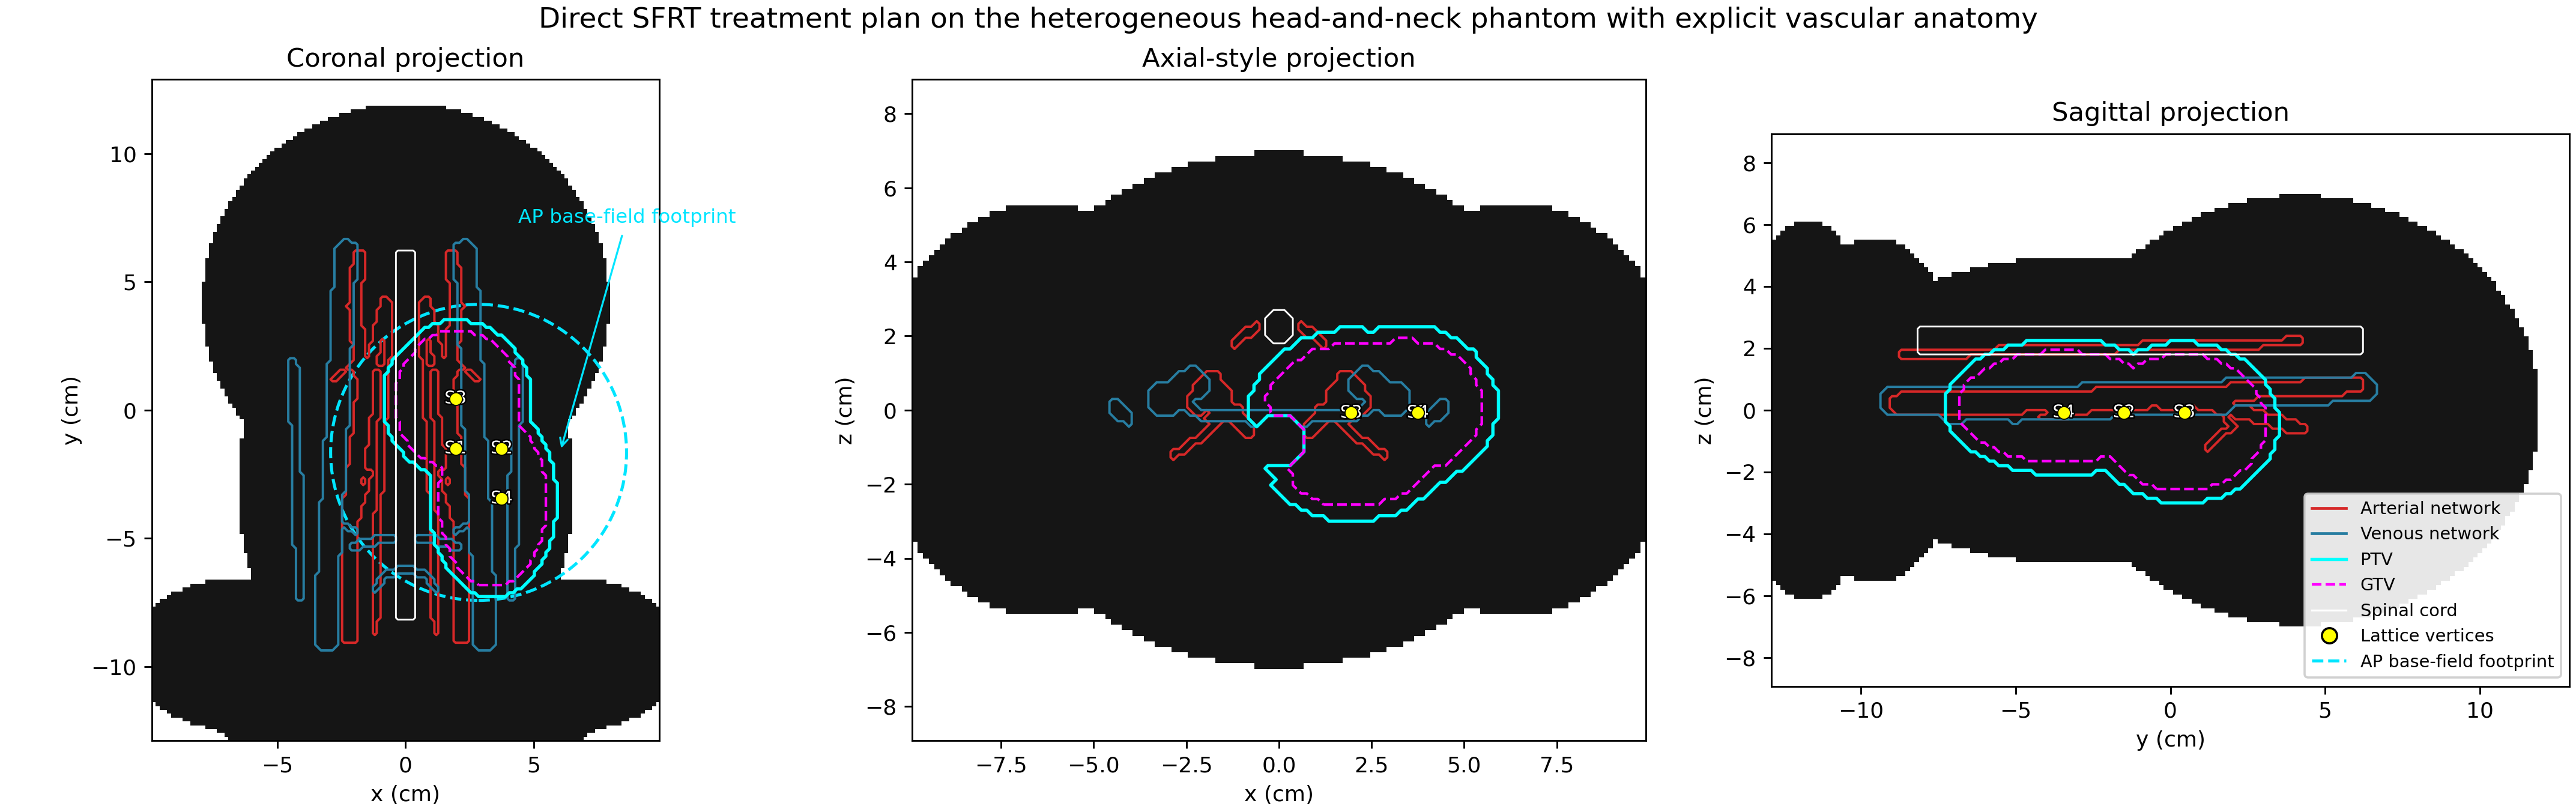
\includegraphics[width=\linewidth]{figureM4_treatment_plan_with_vessels.png}
    \caption{\textbf{Direct 3D lattice SFRT plan applied to the heterogeneous voxelized phantom.} The AP base-field footprint, lattice vertices, target contours, spinal cord, and explicit arterial and venous networks are overlaid in orthogonal projections.}
    \label{fig:treatment_plan_with_vessels}
\end{figure}

\begin{figure}[H]
    \centering
    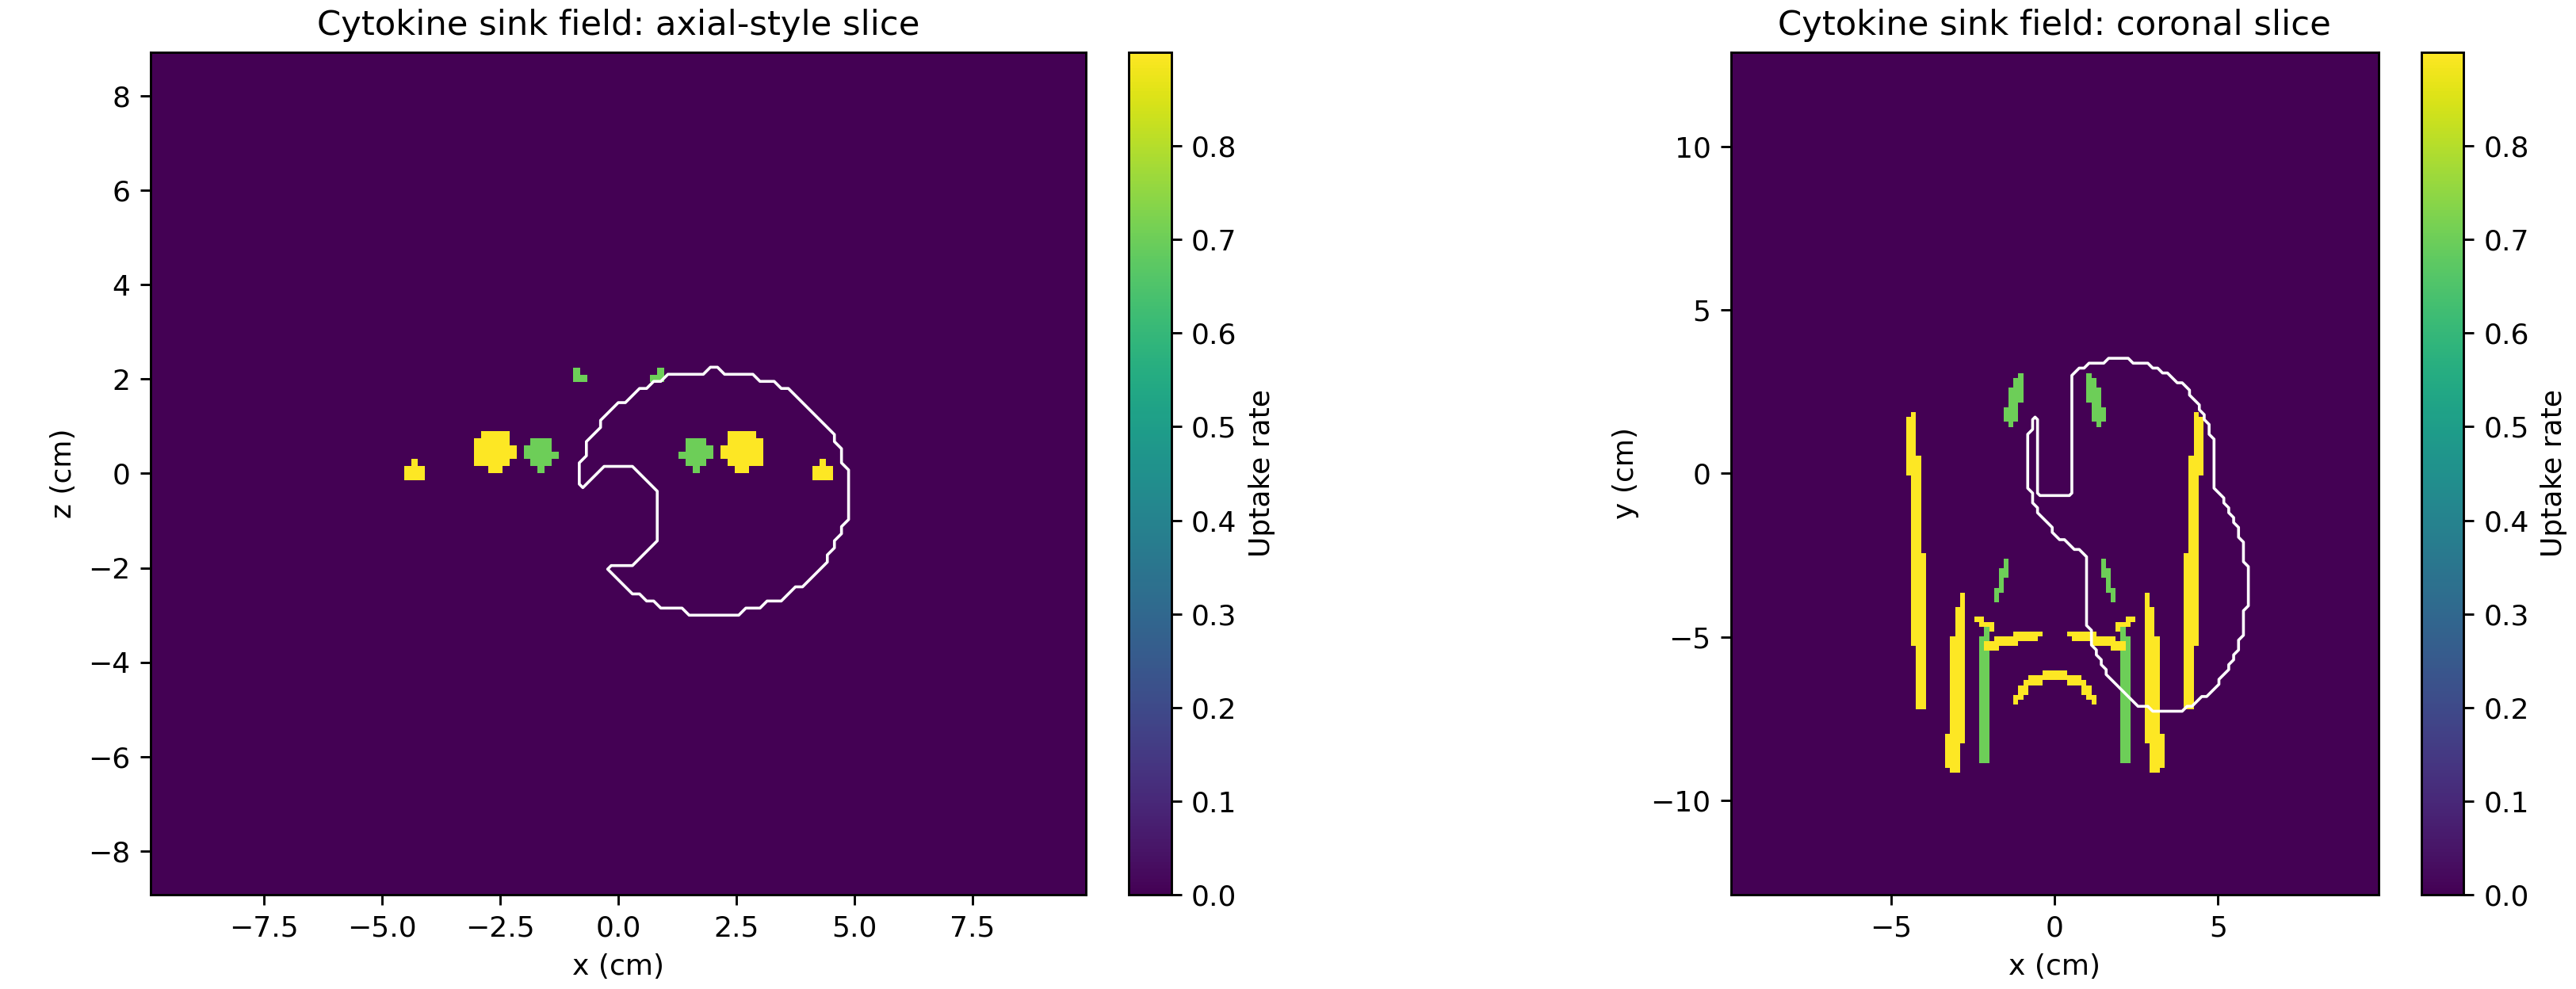
\includegraphics[width=\linewidth]{figureM5_vascular_sink_field.png}
    \caption{\textbf{Anatomical vascular sink field used for the biology-aware reinterpretation.} The cytokine uptake field was derived directly from the explicit arterial and venous voxel masks and used as the spatial washout term in the reaction-diffusion model.}
    \label{fig:vascular_sink_field}
\end{figure}
